% ----------------------------------------------------------------------
%
%        Vorlage für Abschlussarbeiten am Lehrstuhl Informatik VII
%
%                   http://ls7-www.cs.uni-dortmund.de
%
%   Für Fragen und Anregungen zur Vorlage: info@ls7.cs.uni-dortmund.de
%
%   Stand: 07.09.2016
%
% ----------------------------------------------------------------------

\RequirePackage{ifthen}
%
% Arbeitsbezeichnung: Bachelor-Arbeit, Master-Arbeit, Diplomarbeit
%
\newcommand \Arbeitsbezeichnung{Ausarbeitung zum Fachprojekt}
\newcommand \Autor{Marco Greco\\Enes Arpaci\\Vincent Reckendrees\\Artur Ljulin\\ }
\newcommand \Arbeitstitel{Realisierung eines Tennis-Spiels mit Leap-Motion}
\newcommand \Erstgutachter{Dipl.-Ing. Thomas Kehrt}
\newcommand \Zweitgutachter{M.Sc.~Vorname~Nachname}
\newcommand \ErstLehrstuhl{Lehrstuhl Informatik VII}
\newcommand \ErstLehrstuhltitel{Graphische Systeme}

% -----------------------------------------------------------------------------------------
% Option: Zweiter Lehrstuhl
\newboolean{boolkeinZweitLS}
\setboolean{boolkeinZweitLS}{true} % Zuweisung auf ''false'' sofern zweiter Lehrstuhl beteiligt
\ifthenelse{\boolean{boolkeinZweitLS}}{
\newcommand \ZweitLehrstuhl{}
\newcommand \ZweitLehrstuhltitel{}
}{
\newcommand \ZweitLehrstuhl{Lehrstuhl Informatik XII}
\newcommand \ZweitLehrstuhltitel{Eingebettete Systeme}
}

\RequirePackage{ifpdf} \ifpdf
  \pdfoutput=1
  \pdftrue
  \message{pdfLaTeX}
  \documentclass[pdftex,12pt,a4paper,twoside,ngerman,numbers=noenddot]{scrbook}
  \usepackage{float}
  \usepackage[pdftex]{thumbpdf}
  \usepackage[pdftex]{graphicx}
  \usepackage[pdftex]{hyperref}
  \usepackage{pdfpages}
  \pdfoutput=1
  \pdfcompresslevel=9
  \DeclareGraphicsExtensions{.pdf,.jpg,.png}
\else
  \pdffalse
  \message{LaTeX}
  \documentclass[dvips,12pt,a4paper,twoside,ngerman,numbers=noenddot]{scrbook}
  \usepackage{float}
  \usepackage{graphicx}
  \usepackage{epsf}
  \usepackage[dvips]{hyperref}
  \DeclareGraphicsExtensions{.eps}
\fi


% Informationen fuer pdf-File festlegen
\hypersetup
{
    pdfauthor = {\Autor},
    pdftitle = {\Arbeitstitel},
    pdfsubject = {\Arbeitsbezeichnung, TU Dortmund, Fakult{\"a}t f{\"u}r Informatik},
    pdfproducer = {LaTeX},
    pdfview = FitV,
    pdfstartview = FitV,
    pdfhighlight = /I,
    pdfborder = 0 0 0,
    colorlinks = false,
    bookmarksopen,
    bookmarksopenlevel = 1,
    bookmarksnumbered = false,
    plainpages = false
}%


% Seitenformat anpassen
\usepackage[a4paper,left=3.5cm,right=2.5cm,bottom=3.5cm,top=3cm]{geometry}
\setlength{\headheight}{15pt}
% -------------------------------------------------------------------
% Grafikpakete einbinden
\usepackage{amsmath,amssymb}
\usepackage{flafter}
\usepackage{subfigure}

% -------------------------------------------------------------------
\usepackage{ifthen}

% -------------------------------------------------------------------
\usepackage[absolute,overlay]{textpos}
\setlength{\TPHorizModule}{1mm}
\setlength{\TPVertModule}{\TPHorizModule}
\textblockorigin{0mm}{0mm}
\usepackage{fix-cm}
\usepackage{setspace}
\usepackage{scrhack}
% -------------------------------------------------------------------
% Korrekte Darstellung der Umlaute
\usepackage[german,ngerman]{babel}
\usepackage[utf8]{inputenc}
\usepackage[T1]{fontenc}
\usepackage{ae,aecompl}


% -------------------------------------------------------------------
% Bibtex deutsch
\usepackage[numbers,sort]{natbib}


% -------------------------------------------------------------------
% Anführungszeichen
\usepackage[babel,german=quotes]{csquotes}


% -------------------------------------------------------------------
% URLs
\usepackage{url}
% Trennung langer urls
\usepackage[hyphenbreaks]{breakurl}
\def\UrlBreaks{\do\a\do\b\do\c\do\d\do\e\do\f\do\g\do\h\do\i\do\j\do\k\do\l%
\do\m\do\n\do\o\do\p\do\q\do\r\do\s\do\t\do\u\do\v\do\w\do\x\do\y\do\z\do\0%
\do\1\do\2\do\3\do\4\do\5\do\6\do\7\do\8\do\9\do\-}%

% -------------------------------------------------------------------
% Caption anpassen
\usepackage[margin=0pt,font=small,labelfont=bf]{caption}

% -------------------------------------------------------------------
% Erweitere Tabellen
\usepackage{booktabs}

% -------------------------------------------------------------------
% Eurosymbol
\usepackage{eurosym}

% -------------------------------------------------------------------
% Zeilenabstand einstellen
\renewcommand{\baselinestretch}{1.25}
% Floating-Umgebungen anpassen
\renewcommand{\topfraction}{0.9}
\renewcommand{\bottomfraction}{0.8}

% -------------------------------------------------------------------
% Keine einzelnen Zeilen beim Anfang eines Abschnitts (Schusterjungen)
%\clubpenalty = 10000
% Keine einzelnen Zeilen am Ende eines Abschnitts (Hurenkinder)
%\widowpenalty = 10000 \displaywidowpenalty = 10000

\parindent=0cm


% -------------------------------------------------------------------
% Kopfzeile hinzufuegen
\usepackage{fancyhdr}
\usepackage{extramarks}

\pagestyle{fancy}
\renewcommand{\chaptermark}[1]{\markboth{#1}{}}
\renewcommand{\sectionmark}[1]{\markright{#1}{}}

\fancyhf{}
\fancyhead[LE,RO]{\thepage}
\fancyhead[RE]{\textit{\nouppercase{\leftmark}}}
\fancyhead[LO]{\textit{\nouppercase{\rightmark}}}

\fancypagestyle{plain}{ %
\fancyhf{} % remove everything
\renewcommand{\headrulewidth}{0pt} % remove lines as well
\renewcommand{\footrulewidth}{0pt}} \pagestyle{headings}



% -------------------------------------------------------------------
% Eigene Farben definieren
\usepackage{color}
\definecolor{TUGreen}{rgb}{0.517,0.721,0.094}
\definecolor{TUOrange}{rgb}{1.0,0.7176,0.0}
\definecolor{BrightGray}{gray}{0.9}
\definecolor{DarkGray}{gray}{0.2}
\definecolor{white}{rgb}{1,1,1}
\definecolor{black}{rgb}{0,0,0}
\definecolor{red}{rgb}{1,0,0}




% -------------------------------------------------------------------
% Programm-Listings einbinden und formatieren
\usepackage{listings}

\lstdefinestyle{C++}
{
language=C++,
backgroundcolor=\color{BrightGray},
keywordstyle=\texttt\bfseries,  %\color{TUGreen}\bfseries,
commentstyle=\color{DarkGray},
stringstyle=\color{red},
showstringspaces=false,
basicstyle=\small\color{black},
numbers=left,
captionpos=b,
tabsize=4,
breaklines=true
}


% -------------------------------------------------------------------
% Algorithmen
\usepackage[plain,chapter]{algorithm}
\usepackage{algorithmic}

\usepackage{enumerate}

% -------------------------------------------------------------------
% Algorithmen anpassen
\renewcommand{\algorithmicrequire}{\textit{Eingabe:}}
\renewcommand{\algorithmicensure}{\textit{Ausgabe:}}
\floatname{algorithm}{Algorithmus}
\renewcommand{\listalgorithmname}{Algorithmenverzeichnis}
\renewcommand{\algorithmiccomment}[1]{\color{grau}{// #1}}


% -------------------------------------------------------------------
% -------------------------------------------------------------------
% -------------------------------------------------------------------
\begin{document}
\pagenumbering{alpha}

%========================================================================================
% TU Dortmund, Informatik Lehrstuhl VII
%========================================================================================

\begin{titlepage}

\begin{textblock}{150}(30.5,10.75)%
\raggedright

\includegraphics[width=83.25mm]{bilder/tud_logo_cmyk.pdf}%
\end{textblock}

\begin{textblock}{150}(21.2,41.6)%
\raggedright\textsf%\Huge
{\color{red}\rule{5mm}{5mm}}
\end{textblock}

\begin{textblock}{150}(30.4,40.32)%
\raggedright

\includegraphics[width=90mm]{bilder/fi_text.pdf}
\end{textblock}

\begin{textblock}{89}(35.0,62.75)%
\begin{minipage}{80mm}
	\vfill
	\begin{center}
	\fontsize{24pt}{24pt} \textsf
	\Arbeitsbezeichnung
	
	\vspace{1cm}
	\begin{onehalfspace}
    \fontsize{18pt}{18pt}
    \textsf \Arbeitstitel
    \end{onehalfspace}
	
	\vspace{12mm}
\begin{onehalfspace}
	{\fontsize{14pt}{14pt}\textsf \Autor}
 \end{onehalfspace}
\begin{onehalfspace}
	  {\today}
\end{onehalfspace}
	\end{center}
	\vfill
\end{minipage}\end{textblock}

\begin{textblock}{150}(44.25,208)%
\begin{minipage}{120mm}
	\large
	\raggedright
	\textsf
    {\fontsize{14pt}{14pt}
	\textbf{Gutachter:}\\
	\Erstgutachter\\
}
\end{minipage}
\end{textblock}



\begin{textblock}{150}(44.25,242.0)%
\ifthenelse{\boolean{boolkeinZweitLS}}{
%
\begin{minipage}{120mm}
	\fontsize{11.75pt}{11.75pt}\selectfont
	\raggedright
	%\textsf
	\textcolor{TUGreen}{\ErstLehrstuhl}\\
	\textcolor{TUGreen}{\ErstLehrstuhltitel}\\
    \textcolor{TUGreen}{TU Dortmund}
\end{minipage}
%
}{
%
\begin{tabular*}{\textwidth}[t]{c c}%
  \begin{minipage}[t]{70mm}
    \raggedright
	\textsf
    \textcolor{TUGreen}{\ErstLehrstuhl}\\
    \textcolor{TUGreen}{(\ErstLehrstuhltitel)}\\
    \textcolor{TUGreen}{TU Dortmund}
    \end{minipage}
    \hspace*{0.5cm}
    \begin{minipage}[t]{70mm}
    \raggedright
	\textsf
    \textcolor{TUOrange}{\ZweitLehrstuhl}\\
    \textcolor{TUOrange}{(\ZweitLehrstuhltitel)}\\
    \textcolor{TUOrange}{TU Dortmund}
  \end{minipage}
\end{tabular*}
%
}
%
\end{textblock}



\vspace*{20cm}



\end{titlepage}


\pagestyle{empty} \cleardoublepage

\pagenumbering{roman} \tableofcontents

\cleardoublepage \pagestyle{headings}

\pagenumbering{arabic}

% -------------------------------------------------------------------

%\pagestyle{empty}
%%========================================================================================
% TU Dortmund, Informatik Lehrstuhl VII
%========================================================================================

\chapter*{Mathematische Notation} \label{Notation}
\addcontentsline{toc}{chapter}{Mathematische Notation}

\newcommand{\tabdummy}{\midrule[0pt]}

\begin{tabular}{p{0.25\textwidth}p{0.65\textwidth}}
  \textbf{Notation} & \textbf{Bedeutung} \\ \toprule[1pt]
   $\mathbb{N}$ & Menge der natürlichen Zahlen ${1, 2, 3, \ldots}$ \\ \tabdummy
   $\mathbb{R}$ & Menge der reellen Zahlen \\ \tabdummy
   $\mathbb{R}^d$ & $d$-dimensionaler Raum\\ \tabdummy
   $\mathcal{M} = \{m_1,\ldots,m_N\}$ & ungeordnete Menge $\mathcal{M}$ von $N$
   Elementen $m_i$ \\ \tabdummy
   $\mathcal{M} = \langle m_1,\ldots,m_N\rangle$ & geordnete Menge $\mathcal{M}$ von $N$
   Elementen $m_i$ \\ \tabdummy
   $\mathbf{v}$ & Vektor $\mathbf{v}=(v_1,\ldots,v_n)^T$ mit N Elementen $v_i$\\ \tabdummy
   $v^{(j)}_i$ & $i$-tes Element des $j$-ten Vektors\\ \tabdummy
   $\mathbf{A}$ & Matrix $\mathbf{A}$ mit Einträgen $a_{i,j}$\\ \tabdummy
   $G=(V,E)$ & Graph $G$ mit Knotenmenge $V$ und Kantenmenge $E$ \\ \tabdummy

\end{tabular}

%\cleardoublepage

\pagestyle{fancy}

%========================================================================================
% TU Dortmund, Informatik Lehrstuhl VII
%========================================================================================

\chapter{Einleitung}
\label{Einleitung}
1 Einleitung
Das vorliegende Arbeit beschäftigt sich mit dem Abschlussprojekt des Visual Computing Fachprojekts zur Realisierung eines virtuellen Tennis Spiels, bei dem 
die Steuerung durch Leap Motion umgesetzt wird.
In dem Projekt wurden einige Projekte, welche zuvor im Fachprojekt vorgestellt wurden, kombiniert. Hierbei wurde vor allem Leap Motion für die Realisierung des Schlägers genutzt und des weiteren
Grundkenntnisse in OpenGL um die benötigten Objekte zu visualisieren.




\section{Motivation}
\label{Motivation_und_Hintergrund}
%
1.1 Motivation 
Für die letzte Phase des Fachprojekts wurde die Vorgabe gestellt, ein eigenständiges Projekt in einer kleinen Gruppe zu entwickeln, wobei wir dabei
das bereits Gelernte kreativ einsetzen sollten, damit die erlernten Kompentenzen aufgefrischt und gefestigt werden.
Die Idee für die wir uns nach kurzer Beratungszeit entschieden haben sollte ein Tennis Spiel sein, wobei die Hand als Schläger fungiert und die Erkennung der Hand
durch Leap Motion gewährleistet wird. 
Das Projekt besteht aus hinreichend vielen Problemen, welche wir gleichmäßig aufteilten. Die Teilprobleme haben unterteilt in die physikalischen Einflüsse, wobei
wir großen Wert auf einen realistischen Spielfluss gelegt haben, das Rendering, um die gebrauchten Objekte zu erstellen und die Steuerung, welches vorallem die korrekte Erfassung der Hand
beinhaltete. 
Die Regeln des Spieles sind sehr schnell zu erlernen und sprechen jede mögliche Zielgruppe an, da die Regeln leicht verständlich und die Steuerung sehr intuitiv sind. %deswegen haben wir großen Wert auf ein an




\newpage
\section{Problemstellung}
\label{Aufbau_der_Arbeit}
%

Um das Tennis Spiel zu realisieren haben wir uns intensiv mit folgenden drei Teilproblemem beschäfigt. Da sie teilweise nicht aufeinander aufbauten, hat es sich angeboten parallel an denen zu arbeiten.\\
Für die Steuerung des Spiels musste der Leap Motion Kontroller korrekt angebunden werden, sodass zusätzliche Daten bezüglich der Hand gewonnen werden konnte, welche beispielweise für die Ausrichtung des Schlägers wichtig war.
Durch Anbindung des Leap Motion Kontrollers haben wir das Ziel verfolgt die Intuitivität des Spielers anzusprechen, da er zum Spielen lediglich seine Hand braucht.\\
Die Objekte, welche visualisiert werden sollten, mussten gerendert werden. Dies beinhaltete unter anderem eine Box in der das Spiel abläuft, einen Ball und einen Schläger. Außerdem wurden
einige Extras eingebunden, um dem ganzen Projekt mehr Farbe zu geben.\\
Der dritte Themenbereich umfasst die ganze Physik und die Berechnungen welche diese mit sich führt. Dabei haben wir Wert darauf gelegt Faktoren die in der Realität vorhanden sind, wie 
zum Beispiel die Schwerkraft oder ähnliches in unser Projekt zu implementieren, um dem Spieler eben dieses Gefühl von Intuitivität und Realität wiederzugeben. 
Die Kollisionserkennung und Berechnung fällt unter diesen Teilbereich, wobei wieder versucht wurde die genannten Faktoren zu realisieren.




\cleardoublepage
%========================================================================================
% TU Dortmund, Informatik Lehrstuhl VII
%========================================================================================

\chapter{Graphische Ausgabe}
\label{Kapitel 2}
%
In der graphischen Ausgabe der Anwendung sollen alle Objekte dargestellt werden. Zu den darstellbaren Objekten gehören der Ball, der Schläger, das Spielfeld und eine Zielscheibe, wie in Abbildung \ref{fig:gameScene} zu sehen ist.

\begin{figure}[h]
	\centering
	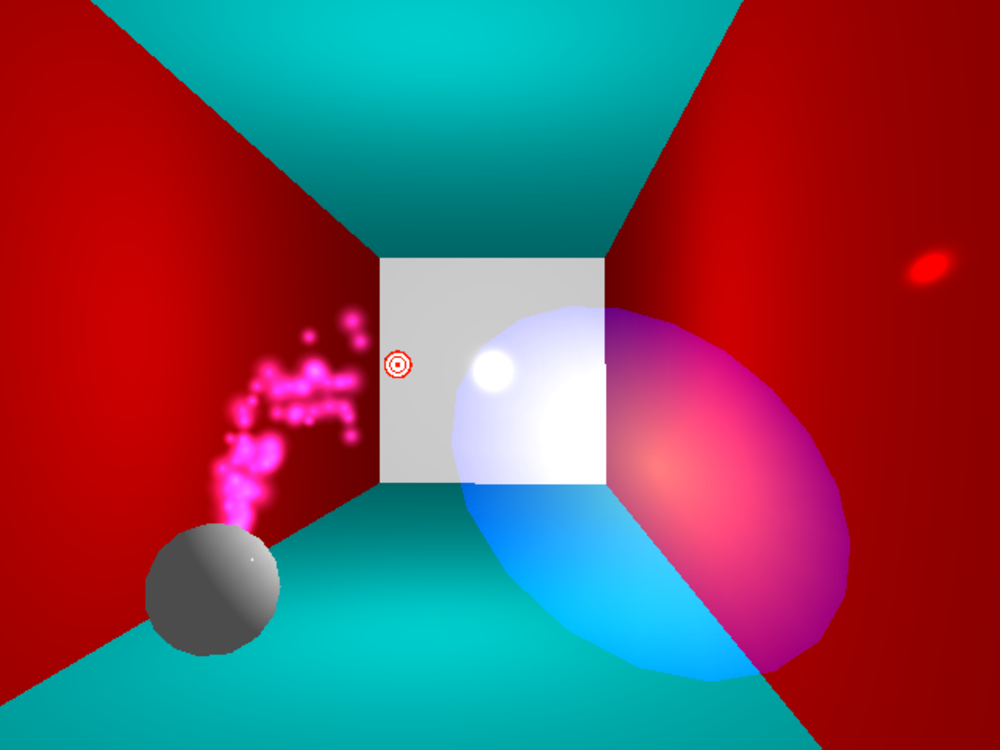
\includegraphics[width=0.6\linewidth]{bilder/gameScene}
	\caption{Szene aus der Anwendung}
	\label{fig:gameScene}
\end{figure}


\section{Rendering Architektur}
\label{Kapitel_2_-_Unterkapitel_1}
%
Der in Abbildung \ref{fig:renderingSystem} dargestellte Ausschnitt des Klassendiagramms (siehe Anhang \ref{anhangA}) zeigt die Klassen des Rendering-Systems und ihre Beziehungen zueinander.

\begin{figure}[h]
	\centering
	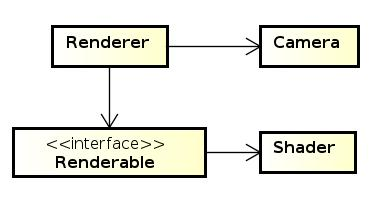
\includegraphics[width=0.6\linewidth]{bilder/RenderingSystem}
	\caption{Klassen des Rendering-Systems}
\label{fig:renderingSystem}
\end{figure}

Der {\texttt{Renderer}} ist die zentrale Klasse des Rendering-Systems und verwaltet eine Liste von {\texttt{Renderable}}s, sowie die {\texttt{Camera}}, die bei jedem Render-Call an die {\texttt{Renderable}}s übergeben wird, damit diese sich die View- und Projection-Matrix holen und gerendert werden können. Damit ein {\texttt{Renderable}} gerendert werden kann besitzt es einen eigenen Shader.

Die Klassen der eingangs erwähnten darstellbaren Objekte, also {\texttt{Ball}}, {\texttt{Racket}}, {\texttt{Box}} und {\texttt{Scorefield}}, enthalten Member, die das {\texttt{Renderable}}-Interface implementieren. Zu den Klassen die das Interface implementieren gehören {\texttt{BallRenderable}}, {\texttt{BallParticleRenderable}},
{\texttt{BoxRenderable}}, {\texttt{RacketRenderable}} und {\texttt{ScorefieldRenderable}}. Innerhalb eines solchen Renderables werden bei der Initialisierung die Buffer für die Render-Daten erzeugt, es werden die Render-Daten an die Buffer übergeben und es wird ein Shader-Programm erzeugt. 

\section{3D-Modelle der Renderables}
%
Für das Erstellen der Modelle, die in der Anwendung zu sehen sind, wurde keine Modelling-Software verwendet. Da es sich bei den Modellen um einfache geometrische Objekte wie Kugeln, Kreise, und Rechtecke handelt, werden die Render-Daten, also Vertizes, Normale, Farben und ggfs. Indizes für die Faces, innerhalb der Renderables erzeugt.

\section{Kamerabewegung}
%
Um die Flugbahn des Balles besser einschätzen zu können und um ein besseres Gefühl für die
Position des Schlägers innerhalb des Spielfeldes zu erhalten, bewegt sich die Kamera bei Bewegung des Schlägers mit. Die Kamerabewegung ist in Abbildung \ref{fig:camera} dargestellt.

\begin{figure}[t]
	\centering
	\subfigure[Kamera in neutraler Position]
	{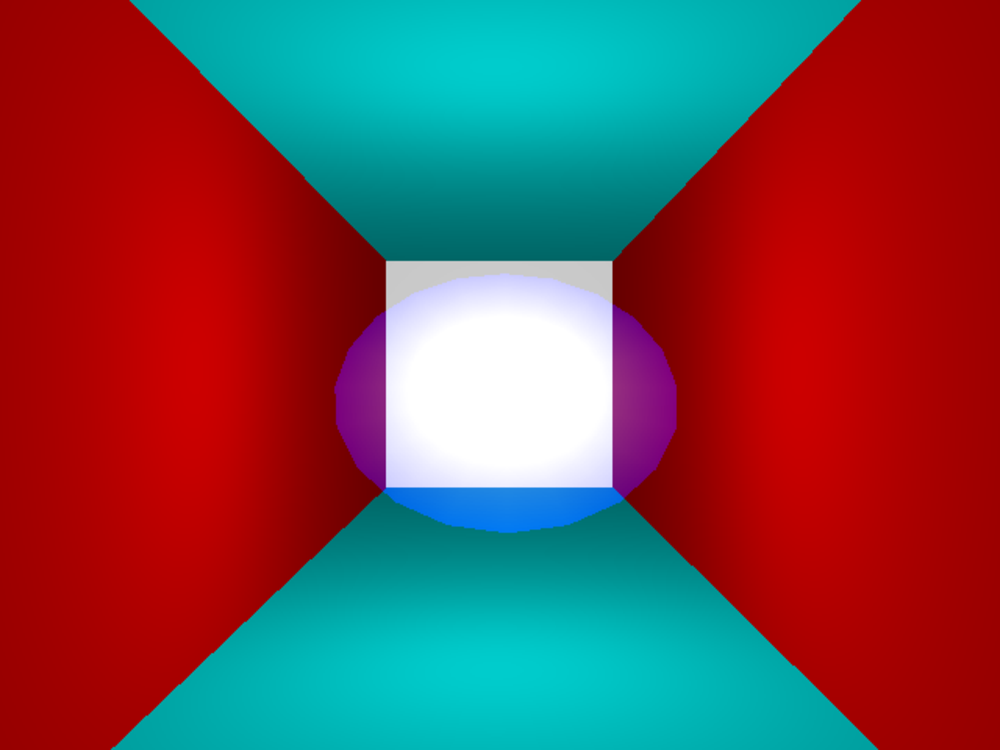
\includegraphics[scale=0.4]{bilder/cameraNeutral}\label{fig:cameraNeutral}
	}
	\vspace{1.5cm}%
	\subfigure[Kamera bei Bewegung des Schlägers nach rechts oben]
	{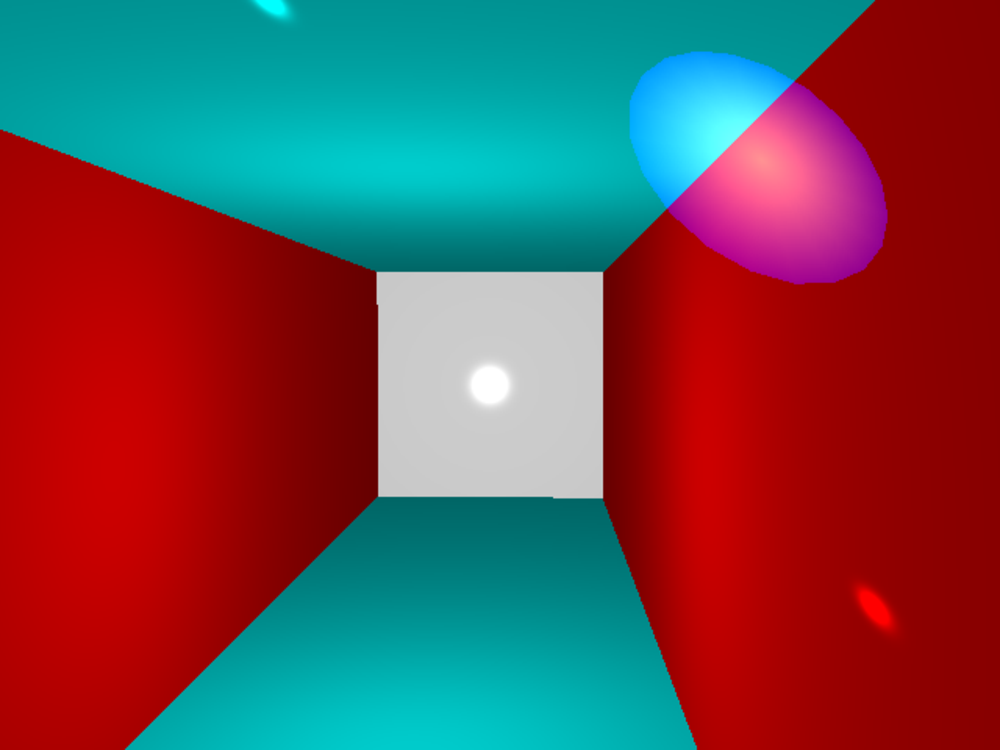
\includegraphics[scale=0.4]{bilder/cameraMoved}\label{fig:cameraMoved}
	}
	\vspace{-1.5cm}
	\caption[Weitere Testbilder]{Kameraposition bei Bewegung des Schlägers}
	\label{fig:camera}
\end{figure}

In jedem Durchlauf der Hauptschleife wird der Kamera nach dem Aktualisieren der Position des Schlägers die neue Position mitgeteilt, wobei nur die $x$- und $y$-Koordinate in die neue Kameraposition mit einfließen. Die Kamera passt dann die View-Matrix an. Der Bewegungsbereich der Kamera ist so eingeschränkt, dass , wenn der Schläger außerhalb dieses Bewegungsbereiches bewegt wird, die Kamera innerhalb des Spielfelds verbleibt.
\section{Partikelsystem}
\label{Kapitel_2_-_Unterkapitel_2}
%
Partikelsysteme sind in interaktiven Anwendungen wie Computerspiele und in der Postproduktion von Filmen, seien es Real- oder Animationsfilme, allgegenwärtig.
Man denke an typische Effekte wie Feuer und Rauch, aber auch Flüssigkeiten lassen sich mithilfe von Partikelsystemen realisieren.

Nach \cite{reeves:particle_systems} sind Partikelsysteme besonders geeignet für Objekte die sich aufgrund ihrer Komplexität nur schwer mit einem Mesh darstellen lassen und sich im Verlauf der Zeit in ihrer Form ändern. Eine einfache Repräsentation solcher Objekte lässt sich daher mit Wolken aus Partikeln umsetzen, wobei die Partikel einfache Primitive wie Punkte, Linien und Dreiecke sind\cite{reeves:particle_systems}.

In der Anwendung wird ein Partikelsystem genutzt um den Flugverlauf des Balles darzustellen. Dabei sind die Partikel Quads, bestehend aus jeweils 6 Vertices, auf die eine Textur projiziert wird.

\subsection{Komponenenten des Partikelsystems}
\label{Kapitel_2_-_Unterkapitel_2.1}
%
In der Anwendung besteht das Partikelsystem aus zwei Klassen, nämlich dem {\texttt{Particle}} und dem {\texttt{BallParticleRenderable}}.

Die {\texttt{Particle}} Klasse repräsentiert ein Partikel, welches eine Position in Weltkoordinaten, eine Geschwindigkeit, eine Lebensdauer und eine Größe hat. 
Die {\texttt{BallParticleRenderable}} Klasse ist für die Darstellung und Verwaltung aller im System vorhandenen Partikel zuständig. Zur Verwaltung gehört das emittieren neuer Partikel, das Aktualisieren der aktiven Partikel und Löschen der ‚toten‘ Partikel, also solcher, deren Lebensdauer null erreicht hat. Die Klasse hält Attribute, die die maximale Anzahl der aktiven Partikel beschränkt sowie die Emittiergeschwindigkeit.  Sie hat auch ein Attribut für die Position. Alle neuen Partikel werden relativ zu dieser Position emittiert. Dabei ist die Position des Emittierpunktes auf dem Rand des Balles entgegengesetzt dem Geschwindigkeitsvektor des Balles.

\subsection{Instanced Rendering}
\label{Kapitel_2_-_Unterkapitel_2.2}
%
Instanced Rendering bezeichnet eine effiziente Variante des Renderns von Objekten die dieselben Renderdaten verwenden, sich aber nur darin unterscheiden, wo sie im Weltkoordinatensystem platziert werden. Für die Partikel unseres Partikelsystems trifft dies zu, da jedes Partikel, wie bereits erwähnt, ein einfaches Quad ist und sich nur in seiner Position und Größe unterscheidet.

Die Effizienz dieser Methode rührt daher, dass zum Rendern der Partikel nun nicht mehr über die Liste aller Partikel iteriert wird und für jedes Partikel ein Draw-Call getätigt wird. Stattdessen wird pro Frame nur ein einziger Draw-Call getätigt, das heißt, dass nur ein Befehl über den langsamen Peripheriebus zur Grafikkarte gesendet werden muss. Für das Instanced Rendering bietet OpenGL die Funktionen {\texttt{glDrawArraysInstanced}} und {\texttt{glDrawElementsInstanced}}.

Um nicht zu sehr in den technischen Details zu versinken, soll nur kurz schematisch anhand von Abbildung \ref{fig:vao} der Vorgang beim Rendern der Partikel erläutert werden.
%Todo vao bild;kurz auf performance eingehen; verweis auf super bible

\begin{figure}[h]
	\centering
	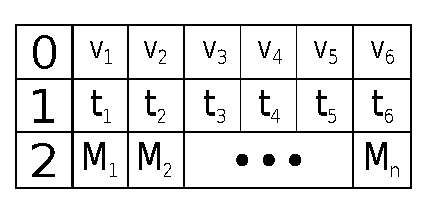
\includegraphics[scale=0.8]{bilder/vao}
	\caption{VAO im {\texttt{BallParticleRenderable}} nach jedem Update der Partikel}
	\label{fig:vao}
\end{figure}

Wie an Abbildung \ref{fig:vao} zu sehen ist, befinden sich die Vertizes $v_1\dotsc v_6$ , die Texturkoordinaten $t_1\dotsc t_6$ und die Model-Matrizen $M_1\dotsc M_n$, wobei $\mathnormal{n}$ die Anzahl der aktiven Partikel ist, in ihren eigenen Array-Buffer. Die Vertices und Texturkoordinaten ändern sich nicht. Die Model-Matrizen hingegen werden bei jedem Update der Partikel neu erzeugt und an den Array-Buffer gesendet.

Um Instanced Rendering zu nutzen muss der Array-Buffer der Model-Matrizen als Instance-Attribut des Vertex-Shaders deklariert werden. Dies sollte bei der Assoziation der Array-Buffer mit den Attributen des Vertex-Shader-Programms geschehen.
Beim Rendern einer Instanz werden nun alle Vertexdaten und Texturkoordinaten, die keine Instanz-Variablen sind, und die jeweilige Model-Matrix der Instanz verwendet.

Für weitere Informationen zum Thema Instanced Rendering sei auf \cite{ksls:2013} verwiesen.

\subsection{Blending und Tiefentest}
\label{Kapitel_2_-_Unterkapitel_2.3}
%
In dem verwendeten Partikelsystem sollen die Farben der Partikel, wenn sie sich überlagern, addiert werden. Der resultierende Effekt ist, dass bei genügend sich überlagernden Partikel ein leuchtend weißer Bereich zu sehen ist. Blending erlaubt es, Farben miteinander zu vermischen und ist ein Teil der Verarbeitung der Fragmente in der Rendering Pipeline. OpenGL bietet verschiedene Blending-Arten an, die durch den Aufruf der Funktion {\texttt{glBlendFunc}} eingestellt werden können. 

\begin{figure}[h]
\centering
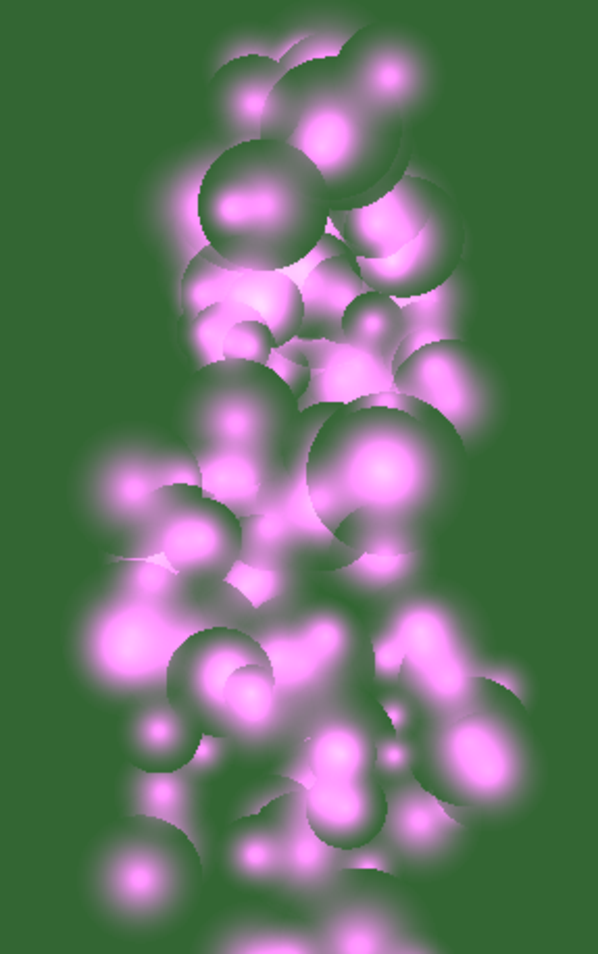
\includegraphics[scale=0.4]{bilder/BlendingEnabled}
\caption{Partikelsystem bei aktiviertem Blending}
\label{fig:BlendingEnabled}
\end{figure}

Abbildung \ref{fig:BlendingEnabled} zeigt wie das Partikelsystem bei eingeschaltetem Blending und Verwendung von {\texttt{glBlendFunc}} mit den Argumenten {\texttt{GL\_SRC\_ALPHA}} und {\texttt{GL\_ONE}} aussieht. Eine Übersicht über die verschiedenen Argumente für {\texttt{glBlendFunc}} und ihre Auswirkungen auf die Farbe eines Fragments ist in \cite{virag:2012} zu finden.

Wie an Abbildung \ref{fig:BlendingEnabled} zu erkennen ist tritt trotz eingeschaltetem Blending der gewünschte Effekt nicht auf. Grund dafür ist der Tiefentest. Für den Tiefentest spielt es keine Rolle, ob ein Fragment teilweise transparent ist, da der Tiefenwert für ein Fragment trotzdem in den Tiefenpuffer geschrieben wird, vorausgesetzt der Wert ist geringer.

Um dies zu umgehen, lässt sich mittels der Funktion {\texttt{glDepthMask}} das Schreiben in den Tiefenpuffer für das Rendern der Partikel verbieten.
Das endgültige Resultat ist in Abbildung \ref{fig:ParticleFinal} zu sehen.

\begin{figure}[h]
	\centering
	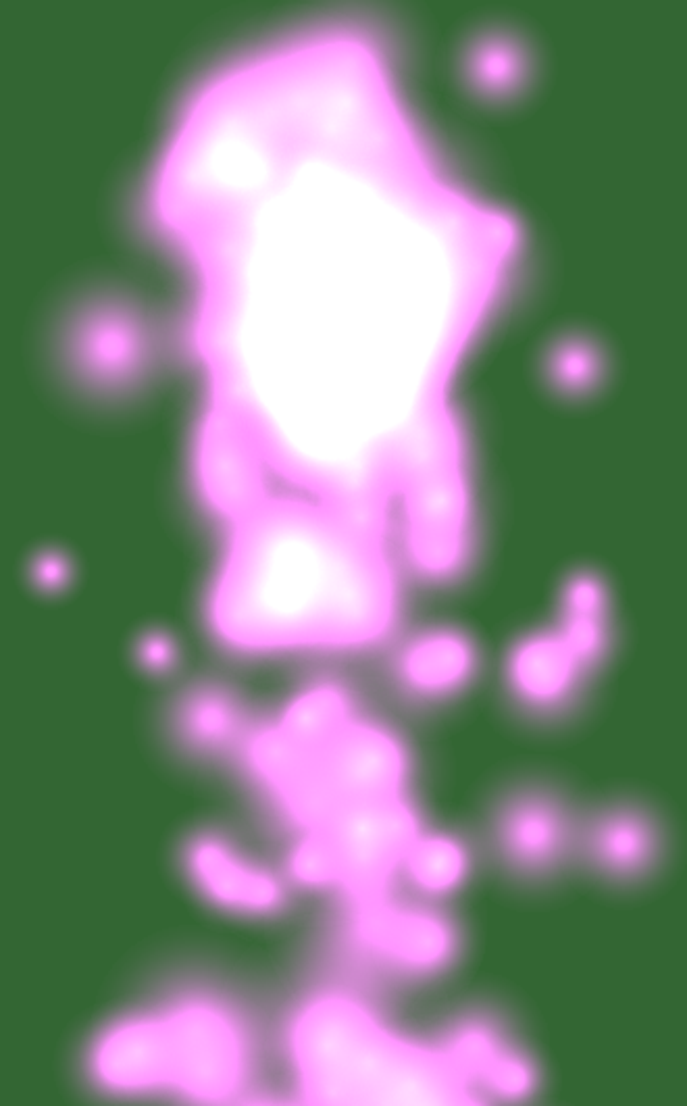
\includegraphics[scale=0.4]{bilder/ParticleFinal}
	\caption{Partikelsystem bei aktiviertem Blending und nicht-beschreibbarem Tiefenpuffer}
	\label{fig:ParticleFinal}
\end{figure}
%


\iffalse
\subsection{Billboarding}
\label{Kapitel_2_-_Unterkapitel_2.4}
%
Für ein besseres visuelles Ergebnis werden die Quads, auf die die Partikeltextur projiziert werden, immer orthogonal zur Blickrichtung der Kamera gerendert. Die Quads erfahren durch die
Modelview-Matrix keinerlei Rotationen. Um diesen Effekt, der als Billboarding bezeichnet wird, zu erreichen muss der Rotationsanteil der View-Matrix, also die linke obere 3x3-Matrix, auf die Einheitsmatrix gesetzt werden.

(Hier Abbildung ohne Billboarding)

Rotationsmatrizen sind Orthogonalmatrizen, das heißt, dass ihre Inversen ihren Transponierten entsprechen. Es genügt also beim Berechnen der Modelview-Matrix die obere linke 3x3-Matrix der Model-Matrix durch die Transponierte des Rotationsanteils der View-Matrix zu ersetzen. Da die Partikel in unserem System auch eine Größe haben wird die resultierende ModelView-Matrix noch mit einer Skalierungsmatrix multipliziert.
\fi

\cleardoublepage
%========================================================================================
% TU Dortmund, Informatik Lehrstuhl VII
%========================================================================================

\chapter{Steuerung}
\label{Kapitel 3}
%
Die Leap Motion bietet über ihre Tracking API (siehe \cite{leap}) die Möglichkeit auf einzelne Daten der durch den Sensor detektierten Hände zuzugreifen. Da der Schläger im Spiel mit der rechten Hand gesteuert wird, werden nur die Position, der Normalenvektor der Handfläche und der Geschwindigkeitsvektor der rechten Hand benötigt.

Die Position der Hand wird zur Bestimmung der Position des Schlägers in der 3D-Szene verwendet. Der Normalenvektor wird zum einen für die Ausrichtung des Schläger-Modells und zum anderen für die Reflexion des Balles bei Kollision mit dem Schläger verwendet. Kommt es zwischen dem Ball und dem Schläger zur Kollision, so wird der Geschwindigkeitsvektor der Hand auf den Geschwindigkeitsvektor des Balles addiert.

Die Leap Motion erlaubt es Gesten zu registrieren, die von der Leap Motion Software erkannt werden können. Im Spiel wird für die linke Hand die Kreisgeste verwendet, die dem Spieler erlaubt den Ball in die Mitte des Spielfelds zurückzusetzen.
%


\cleardoublepage
%========================================================================================
% TU Dortmund, Informatik Lehrstuhl VII
%========================================================================================
\chapter{Physik}
\label{Kapitel 4}

Um die Bewegungen des Ball möglichst realistisch und nachvollziehbar zu realisieren und somit dem Nutzer ein echtes Spielgefühl zu vermitteln, müssen einige physikalische Eigenschaften der "{}echten Welt"{} ins Spiel implementiert werden. In diesem Fall heißt es, dass die Reflexionen eines Balls auf einer Oberfläche richtig berechnet werden müssen. Dementsprechend müssen auch Kollisionsabfragen dafür realisiert werden. Des Weiteren soll die Bewegung des Balls innerhalb der Box korrekt berechnet werden sowie ein Gravitationsfaktor die Fallgeschwindigkeit beeinflussen können.

Da im Programm in jedem Durchlauf der Hauptschleife zuerst die Bewegungen und dann die Kollisionen bzw. die Reflexionen berechnet werden, wird auch in diesem Kapitel diese Reihenfolge beibehalten.
\section{Bewegungen}
\label{Kapitel_4_-_Unterkapitel_1}
Die verschiedenen physikalischen Eigenschaften des Balls werden in der Klasse {\texttt{BallPhysics}} verwaltet. Dazu gehören: Masse, Kraft, Gravitation und Geschwindigkeit.
%====================Kraft wird nicht benutzt!!================
%===================Wahrscheinlich noch ändern=================
Bei jedem Tick wird die Update-Methode des Balls aufgerufen, die wiederum für die Positionsbestimmung zunächst die Update-Methode der Klasse {\texttt{BallPhysics}} aufruft, die die aktuelle Geschwindigkeit berechnet. Da die Geschwindigkeit als 3-dimensionaler Vektor gespeichert wird, ergibt sich daraus auch immer die Richtung in die der Ball sich bewegt. Dabei wird zunächst die Beschleunigung des Balls $\mathbf{a}$, die durch die Gravitationskraft $\mathbf{g}$ beeinflusst wird, berechnet und schließlich auf den Geschwindigkeitsvektor $\mathbf{v}$ addiert.
 \begin{equation}
	    \label{beschleunigung}
	    \mathbf{a} = \mathbf{g} \cdot \Delta t 
    \end{equation}
Mithilfe des Geschwindigkeitsvektor lässt sich dann die nächste Position des Balls bestimmen:
\begin{equation}
	    \label{position}
	   \mathbf{p}_{t+1} = \mathbf{p}_{t} + \mathbf{v} \cdot \Delta t 
    \end{equation}
Schließlich werden dann basierend auf der neuen Position die Rendering-Informationen aktualisiert. 


\section{Reflexion}
\label{Kapitel_4_-_Unterkapitel_2}

Nachdem die Positionen aktualisiert wurden, wird geprüft, ob an den neuen Positionen Kollisionen aufgetreten sind. Dies geschieht in der {\texttt{CollisionResolver}}-Klasse. Die Funktion {\texttt{resolveCollisions(Ball* ball, Racket* racket, Box* box)}} wird von der Hauptschleife aus aufgerufen und überprüft zuerst die Kollision des Balls mit der Box bzw. mit den 6 Ebenen der Box und dann die Kollision mit dem Schläger.
Die Ebenen werden in einer Hesseschen Normalform ähnlichen Darstellung gespeichert, sodass der Abstand des Balls zu einer Ebene leicht berechnet werden kann.

%\begin{figure}[h]
 %   \subfigure[]
%          {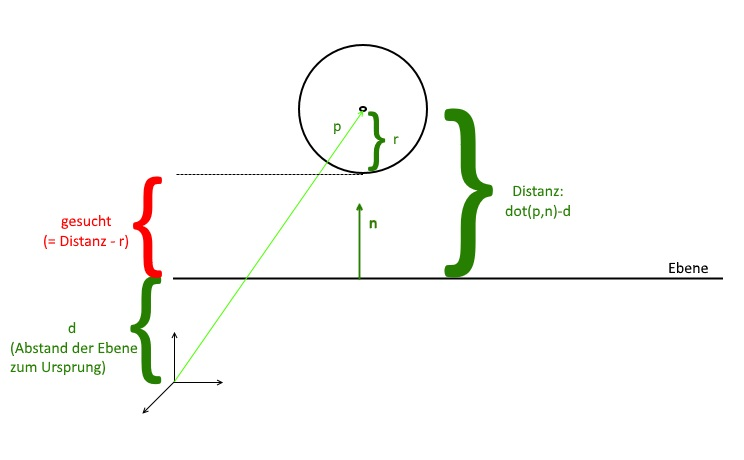
\includegraphics[scale=0.8]{bilder/collision}\label{fig_testbild_a}
%    }
%    \caption{Übersicht der Kollisionsüberprüfung}
%        \label{fig_testbild}
%\end{figure} 

Da die Hessesche Normalform wie folgt aussieht, $ E: \vec x \cdot \vec n  = d $, und d der Abstand zum Ursprung ist, lässt sich die Formel umformen zu $ E: \vec x \cdot \vec n  - d = 0$. Diese Formel ist erfüllt wenn $\vec x$ auf der Ebene liegt. Ersetzt man also 0 durch eine Variable $c$, kann der Abstand von Punkt $\vec x$ zur Ebene genau ermittelt werden. In unserem Fall erlauben wir auch negative Abstände; negative Abstände entstehen dann durch Ballpositionen, die hinter der Ebene liegen (entgegen der Richtung des Normalenvektors).
Der Abstand des Ballmittelpunkts zur Ebene ist also $c = \vec p\cdot \vec n - d $. Somit lässt sich eine Kollision feststellen, wenn der Abstand zur Ebene kleiner als der Radius des Balls ist.

Damit der Ball bei zu hohen Geschwindigkeiten nicht hinter die Ebene gelangt und die Kollision nicht erkannt wird, wurde eine Kollisionsüberprüfung implementiert, die genau dies verhindern soll (nach \cite{migGom:1999}). Denn bei dieser Methode wird der Ball auf eine Position vor der Ebene zurückgesetzt, falls er tatsächlich hinter die Ebene gelangt (s. Abbildung \ref{fig_interpol}). 

Dabei werden immer die letzten beiden Positionen des Balls gespeichert ($\mathbf{p}_t$, $\mathbf{p}_{t-1}$) und die Distanzen zu beiden Zeitpunkten nach schon beschriebener Weise berechnet ($d_t, d_{t-1}$).
Befindet sich $\mathbf{p}_{t-1}$ vor der Ebene und $\mathbf{p}_t$ hinter der Ebene bzw. ist $d_{t-1}$ positiv und $d_t$ negativ, so wird die neue Position des Balls zwischen diesen beiden Punkten interpoliert (s. Formel \ref{interpolEquation1} und \ref{interpolEquation2}). 
\begin{equation}	
\label{interpolEquation1}
	u = \frac{d_{t-1} - R}{d_{t-1} - d_t}
\end{equation}
\begin{equation}	
\label{interpolEquation2}
	\mathbf{p}_{neu} = (1-u)\mathbf{p}_{t-1} + u\mathbf{p}_t
\end{equation}

\begin{figure}[h]
   \begin{center}
       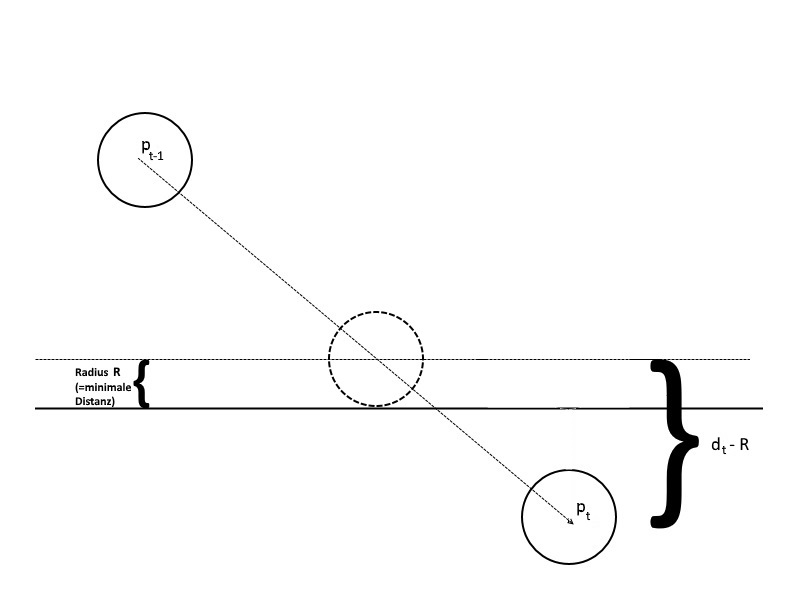
\includegraphics[scale=0.5]{bilder/interpolation}\label{fig_interpolation}
   \end{center}
    
    \caption{Interpolation der Ballposition bei vollständigem Durchstoßen der Ebene}
        \label{fig_interpol}
\end{figure} 

Ist der Ball nicht vollständig hinter die Ebene geflogen - d.h. es gilt $d_t<0$ und $|d_t|<R $ - dann wird der Ball um $R - |d_t|$ in Richtung des Normalenvektors der Ebene verschoben.

Die Kollisionserkennung mit dem Schläger läuft nach ähnlichem Schema ab. Auch die Fläche des Schlägers wird als Ebene gespeichert. Es muss also auch nur der Abstand zu Ebene berechnet werden und mit dem Radius des Balls verglichen werden (visualisiert in Abbildung \ref{fig_colRacket2}). Ist der Abstand kleiner gleich dem Radius, dann kollidiert der Ball mit dem Schläger. Jedoch ist der Schläger keine unendlich große Fläche wie die  Boxwände, sondern ist auf eine bestimmte Kreisfläche begrenzt. Das heißt, dass eine zusätzliche Abfrage gemacht werden muss, die überprüft, ob der Ball eine entsprechend kleine Distanz zum Schlägermittelpunkt besitzt.
Wenn $\mathbf{p}_{racket}$ die Position des Schlägermittelpunkts, $\mathbf{p}$ die Position des Balls und $R$ den Radius des Schlägers beschreibt, dann gilt bei einer Kollision:
\begin{equation}
	|\mathbf{p}_{racket}\cdot\mathbf{p}| \leq R
\end{equation}

\begin{figure}[h]
   \begin{center}
    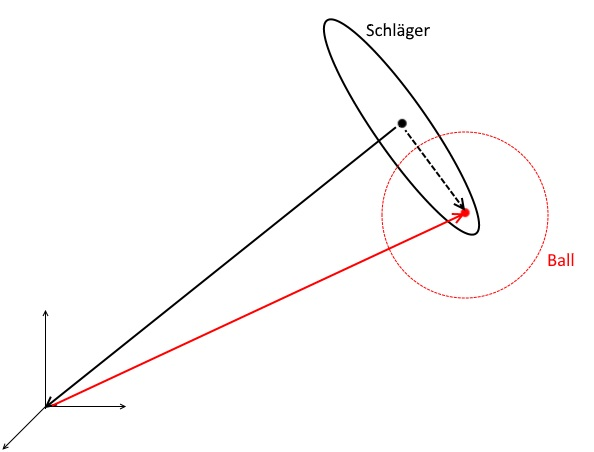
\includegraphics[scale=0.4]{bilder/collisionRacket}\label{fig_colRacket}
   \end{center} 
    \caption{Kollisionserkennung zwischen Schläger und Ball}
        \label{fig_colRacket2}
\end{figure} 

Ist eine Kollision aufgetreten, so kann der Ball entsprechend der Formel \ref{reflexion} reflektiert werden.

\begin{equation}	
\label{reflexion}
	\vec{v}_{neu} = 2 \cdot \langle \vec{n},-\vec{v} \rangle \cdot \vec{n} + \vec{v}
\end{equation}

Um den neuen Vektor zu berechnen muss zunächst der Einfallsvektor des Balls auf den Normalenvektor projiziert werden (gesucht ist also ein Faktor $k$, sodass $k\vec{n}$ eine Projektion von $-\vec{v}$ nach $\vec{n}$ ist). Der Einfallsvektor wird deswegen invertiert, weil ein Ausfallsvektor gesucht wird, der nicht wie der Einfallsvektor in Richtung der Ebene zeigt. $k$ lässt sich mithilfe des Skalarprodukts $\langle\vec{n},-\vec{v}\rangle$ berechnen, da der Normalenvektor einer Ebene in unserer Implementierung immer normiert gespeichert wird.



    \begin{figure}
	\begin{center}
    \subfigure[Projektion des Einfallsvektors auf den Normalvektor]
          {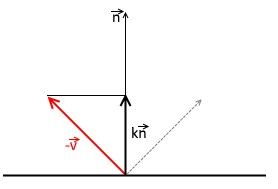
\includegraphics[scale=0.8]{bilder/reflexion1}\label{fig_reflexion_a}
    }
    \hspace{1.5cm}%
    \subfigure[Zusammensetzung des Ausfallsvektors]
         {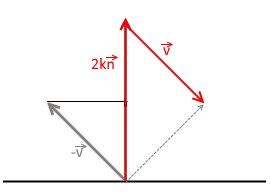
\includegraphics[scale=0.8]{bilder/reflexion2}\label{fig_reflexion_b}
    }
    \caption{Berechnung des neuen Vektors bei einer Reflexion an einer Ebene mit Normalenvektor}
        \label{fig_reflexion}
	\end{center}
    \end{figure}
    
Die Länge des projizierten Vektors $k\vec{n}$ muss nun, wie in Abbildung \ref{fig_reflexion_b} zu sehen, verdoppelt werden und zum Einfallsvektors $\vec{v}$ addiert werden. Das Ergebnis ist dann der Ausfallwinkel in entsprechender Richtung. Soll der Ausfallsvektor betragsmäßig kleiner sein (d.h. der Ball soll z.B. beim Abprallen an Wänden an Geschwindigkeit verlieren), kann der Vorfaktor 2 entsprechend verringert werden (In unserer Implementierung beträgt der Wert: 1,75).

\cleardoublepage
%========================================================================================
% TU Dortmund, Informatik Lehrstuhl VII
%========================================================================================

\chapter{Ergebnisse und Diskussion}
\label{Kapitel 5}
%
Um die Umsetzung des Fachprojekts zu analysieren und ausreichend zu diskutieren, wurden Testpersonen befragt, nachdem sie eine Zeit lang das Spiel getestet haben. Folgende Fragen wurden ihnen danach gestellt:
\begin{enumerate}
	\item \glqq Welche Probleme haben Sie bei der Steuerung bemerkt ?\grqq
	\item \glqq Wie haben Sie die Steuerung im Vergleich zum normalen Tischtennis empfunden ?\grqq
	\item \glqq Als wie realitätsnah haben Sie die Bewegung des Balls empfunden ?\grqq
	
\end{enumerate}

\section{Graphische Ausgabe}
\label{Kapitel_5_-_Unterkapitel_1}
Die graphische Ausgabe wurde von allen Testpersonen für gut empfunden. Probleme, die bei der Steuerung auftraten,  wurden durch die Kamerabewegung beim Bewegen der Hand und die nahe Ansicht auf die Szene verstärkt. Eine Testperson antwortete auf Frage eins: \glqq Da die Kamera sich mit der Hand bewegt, ist es manchmal schwer den Ball zu treffen.\grqq. Die Bewegung der Kamera wäre nicht notwendig, wenn die Szene aus größerer Entfernung betrachtet werden würde.
\section{Steuerung}
\label{Kapitel_5_-_Unterkapitel_2}
Beim Bedienen der Anwendung traten  die meisten Probleme auf. Eine Person antwortete auf Frage zwei: \glqq Das tatsächliche Gefühl, Tischtennis zu spielen, ist nicht vorhanden. Der Ball wird mit der flachen Hand geschlagen, nicht mit einem Objekt, was in der Hand gehalten wird.\grqq \ Zur Bestimmung der Position des Schlägers sollte nicht der Handmittelpunkt, sondern der Mittelpunkt eines gedachten Schlägers in der Hand des Spielers verwendet werden. Dadurch könnte der Spieler das Gefühl erhalten, er schlage den Ball mit einem Schläger.
\section{Physik}
\label{Kapitel_5_-_Unterkapitel_3}
Einige Testpersonen empfanden, dass die Geschwindigkeit des Balls nach dem Schlagen zu hoch war und zu schnell abnahm. Um den Flug des Balls noch realistischer zu gestalten, könnte die berechnete Gravitation erhöht werden, außerdem sollte die Geschwindigkeit des Balls nach dem er getroffen wurde geringer sein.

% -------------------------------------------------------------------

\cleardoublepage
\appendix

%========================================================================================
% TU Dortmund, Informatik Lehrstuhl VII
%========================================================================================

\chapter{Klassendiagramm}
%
Abbildung \ref{fig:classDiagram} enthält alle in der Anwendung vorkommenden Klassen. Der Übersichtlichkeit halber, wurden die Funktionen und Member der einzelnen Klasse ausgelassen. 

\begin{figure}[h]
\centering
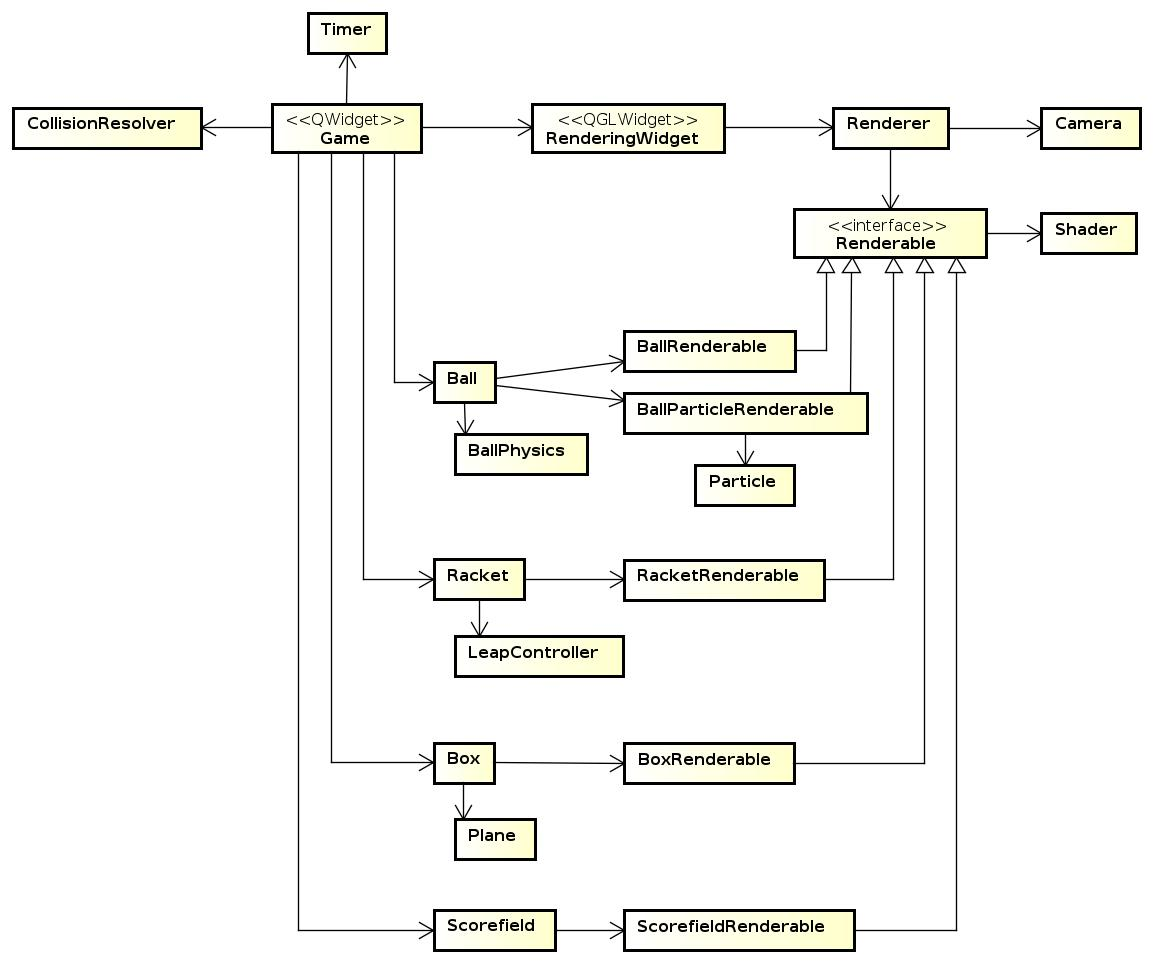
\includegraphics[width=0.9\linewidth]{bilder/classDiagram}
\caption{Klassendiagramm}
\label{fig:classDiagram}
\end{figure}



% -------------------------------------------------------------------

% Abbildungsverzeichnis
\listoffigures
\addcontentsline{toc}{chapter}{Abbildungsverzeichnis}
\cleardoublepage
% Algorithmenverzeichnis
\listofalgorithms
\addcontentsline{toc}{chapter}{Algorithmenverzeichnis}
\cleardoublepage

% Quellcodeverzeichnis
%\renewcommand{\lstlistlistingname}{Quellcodeverzeichnis}
%\lstlistoflistings
%\addcontentsline{toc}{chapter}{Quellcodeverzeichnis}
%\cleardoublepage

% -------------------------------------------------------------------

% Literaturverzeichnis
\addcontentsline{toc}{chapter}{Literaturverzeichnis}
\bibliographystyle{dinatls7}
\bibliography{Literatur}

% -------------------------------------------------------------------

\end{document}
